\documentclass[12pt]{article}
\parindent=.25in

\setlength{\oddsidemargin}{0pt}
\setlength{\textwidth}{440pt}
\setlength{\topmargin}{0in}

\usepackage{amsmath}
\usepackage[dvips]{graphicx}
\usepackage{verbatim}
\usepackage{appendix}

\usepackage{amssymb}
\usepackage{amsfonts}
\usepackage{latexsym}
\usepackage[center]{subfigure}
\usepackage{epsfig}
\usepackage{hyperref}

\title{Stat 4201 Homework 4}
\author{Mengqi Zong $<mz2326@columbia.edu>$}

\begin{document}

\maketitle

\setlength{\parindent}{0in}

\section*{Problem 1}

a. The scatter plot  is shown in Fig~\ref{fig:scatter}.\\

\begin{figure}[ht!]
  \centering
  \includegraphics[width=0.7\textwidth]{scatterplot}
  \caption{Problem 1-a: scatterplot \label{fig:scatter}}
\end{figure}

b. The output of the simple linear regression model from R is shown
below:

\begin{verbatim}
Call:
lm(formula = cesium$Mushrooms ~ cesium$Soils)

Residuals:
    Min      1Q  Median      3Q     Max 
-47.279 -30.319  -9.483  31.000  54.271 

Coefficients:
             Estimate Std. Error t value Pr(>|t|)   
(Intercept)  16.72569   12.41954   1.347  0.19807   
cesium$Soils  0.09590    0.02993   3.205  0.00591 **
---
Signif. codes:  0 ‘***’ 0.001 ‘**’ 0.01 ‘*’ 0.05 ‘.’ 0.1 ‘ ’ 1 

Residual standard error: 36.56 on 15 degrees of freedom
Multiple R-squared: 0.4064,	Adjusted R-squared: 0.3668 
F-statistic: 10.27 on 1 and 15 DF,  p-value: 0.005909 
\end{verbatim}

c. The output of the simple linear regression model excluding sample
number 17 from R is shown below:

\begin{verbatim}
Call:
lm(formula = cesium.trim$Mushrooms ~ cesium.trim$Soils)

Residuals:
    Min      1Q  Median      3Q     Max 
-41.658 -13.938  -4.061   9.744  65.908 

Coefficients:
                  Estimate Std. Error t value Pr(>|t|)   
(Intercept)       43.87726   12.25571   3.580  0.00301 **
cesium.trim$Soils -0.03693    0.04454  -0.829  0.42085   
---
Signif. codes:  0 ‘***’ 0.001 ‘**’ 0.01 ‘*’ 0.05 ‘.’ 0.1 ‘ ’ 1 

Residual standard error: 27.76 on 14 degrees of freedom
Multiple R-squared: 0.04682,	Adjusted R-squared: -0.02126 
F-statistic: 0.6877 on 1 and 14 DF,  p-value: 0.4208 
\end{verbatim}

d. Based on the scatterplot from part a, we can see that example
number 17 is very likely to be an outlier since it is far from every
other samples. After excluding example number 17, we get the linear
model described in part c. Note that this model's R-squared is 0.0468,
which is very close to 0. This indicates that the simple linear
regression model is poorly fitted. From the coefficients' p-value, we
can see that it is very likely that the model is a constant model.\\

In conclusion, there is no linear relationship between Cesium
concentration in soil and Cesium concentration in mushrooms after
Chernobyl accident.\\

e.\\ 

About linearity, based on the R-squared from part b, we can see that
the simple linear regression model is poorly fitted. \\

About normality, I use Shapiro-Wilk normality test on the residuals,
here is the result from R: 

\begin{verbatim}
	Shapiro-Wilk normality test

data:  res.p1 
W = 0.9113, p-value = 0.1053
\end{verbatim}

The p-value is 0.1053. This indicates the data is normal.\\

About homoscedasticity, I use the Residual vs Fitted plot to do the
analysis. The plot is shown in Fig~\ref{fig:p1-RvsF}. Based on the
plot, we can see that the data is not homoscedastic. \\

\begin{figure}[ht!]
  \centering
  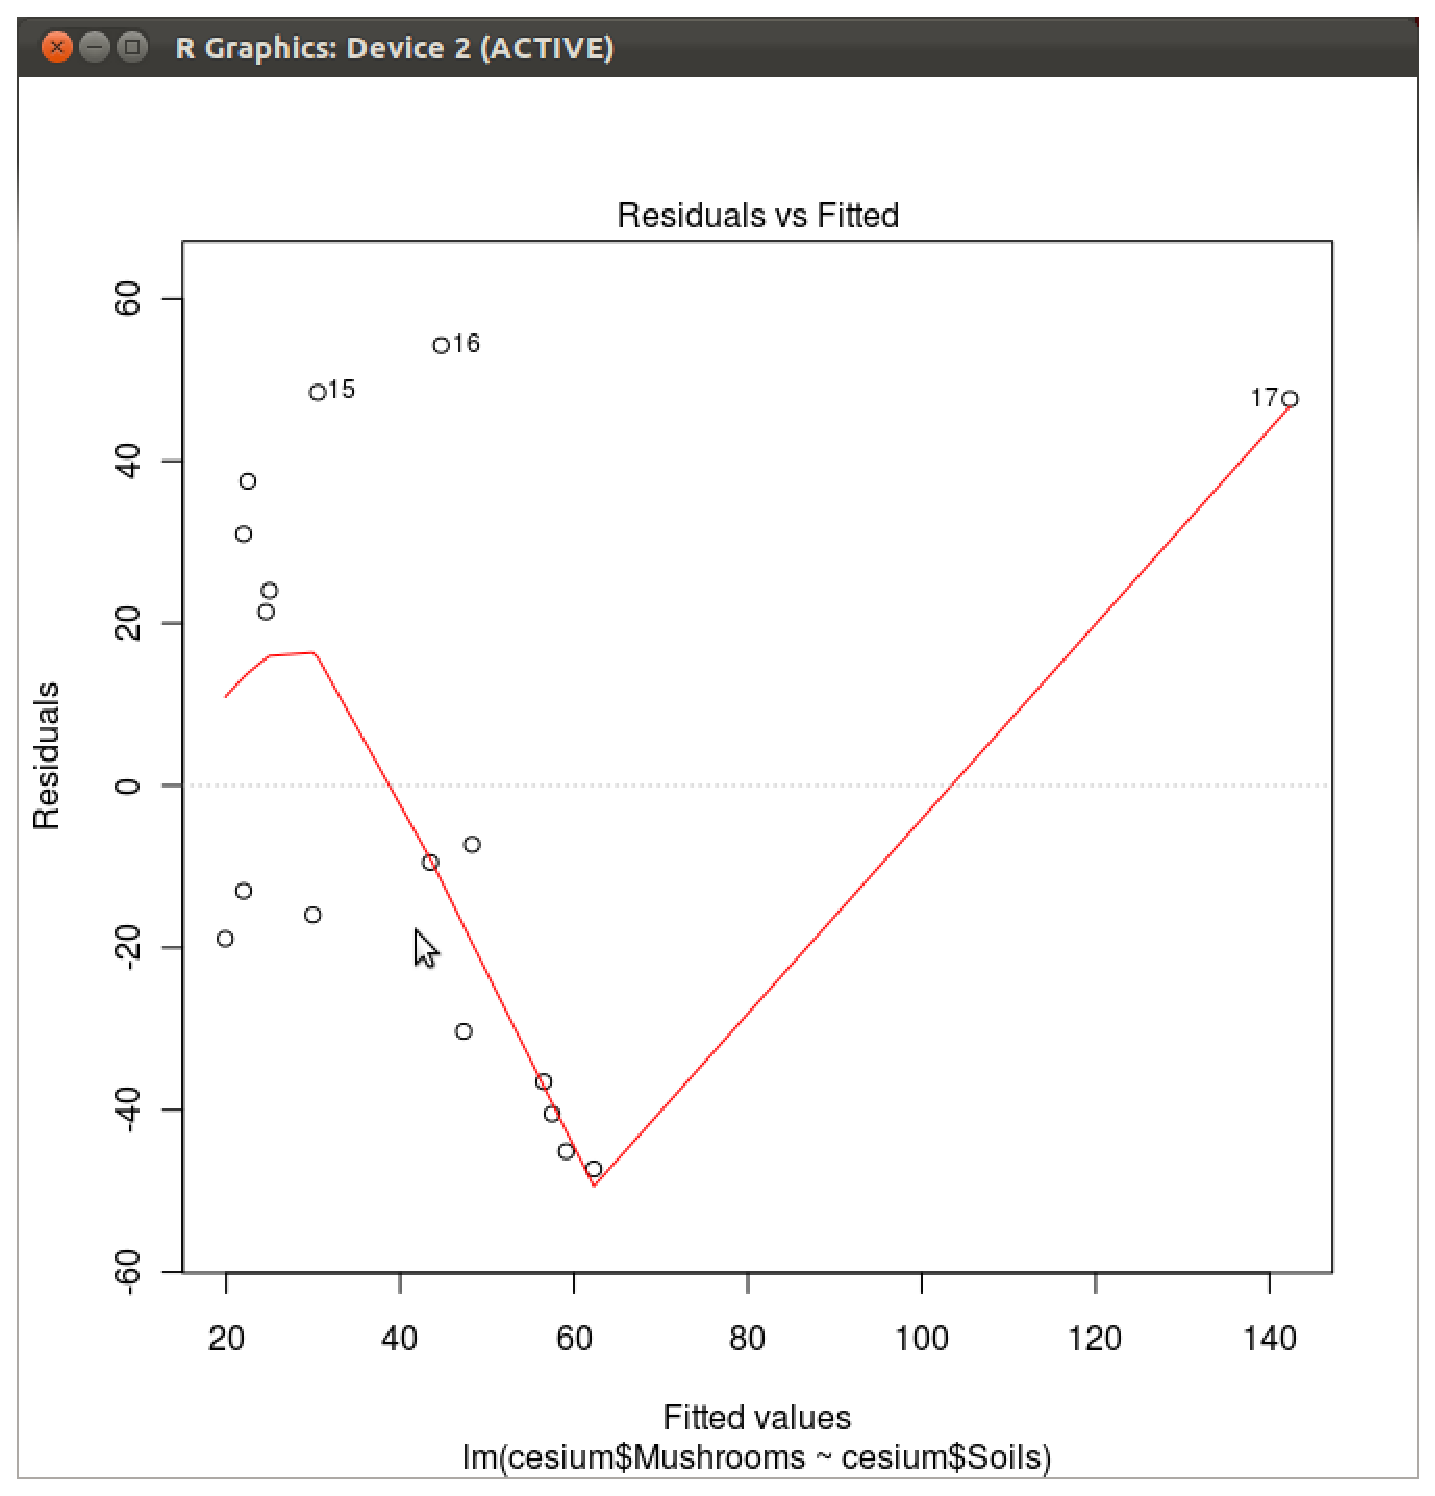
\includegraphics[width=0.7\textwidth]{p1-RvsF}
  \caption{Problem 1-e: Residual vs Fitted \label{fig:p1-RvsF}}
\end{figure}

About uncorrelated error, I use Perason's product-moment test to do
the analysis. And here is the result from R:

\begin{verbatim}
	Pearson's product-moment correlation

data:  cesium$Mushrooms and cesium$Soils 
t = 3.2045, df = 15, p-value = 0.005909
alternative hypothesis: true correlation is not equal to 0 
95 percent confidence interval:
 0.2261250 0.8558834 
sample estimates:
      cor 
0.6374843 
\end{verbatim}

As we can see, Cesium concentrations in mushrooms and soils are
correlated.

\section*{Problem 2}

a. The output of the simple linear regression model from R is shown
below:

\begin{verbatim}
Call:
lm(formula = stack.loss ~ stack.x[, 1] + stack.x[, 2] + stack.x[, 
    3])

Residuals:
    Min      1Q  Median      3Q     Max 
-7.2377 -1.7117 -0.4551  2.3614  5.6978 

Coefficients:
             Estimate Std. Error t value Pr(>|t|)    
(Intercept)  -39.9197    11.8960  -3.356  0.00375 ** 
stack.x[, 1]   0.7156     0.1349   5.307  5.8e-05 ***
stack.x[, 2]   1.2953     0.3680   3.520  0.00263 ** 
stack.x[, 3]  -0.1521     0.1563  -0.973  0.34405    
---
Signif. codes:  0 ‘***’ 0.001 ‘**’ 0.01 ‘*’ 0.05 ‘.’ 0.1 ‘ ’ 1 

Residual standard error: 3.243 on 17 degrees of freedom
Multiple R-squared: 0.9136,	Adjusted R-squared: 0.8983 
F-statistic:  59.9 on 3 and 17 DF,  p-value: 3.016e-09 
\end{verbatim}

b.\\

About linearity, the R-squared for this model is 0,9136. This
indicates that the simple linear regression model is fitted well.\\

About normality, I use Shapiro-Wilk normality test on the residuals,
here is the result from R: 

\begin{verbatim}
	Shapiro-Wilk normality test

data:  e 
W = 0.974, p-value = 0.8186
\end{verbatim}

The p-value is 0.8186. This indicates the data is normal.\\

About homoscedasticity, I use the Residual vs Fitted plot to do the
analysis. The plot is shown in Fig~\ref{fig:p2-RvsF}. Based on the
plot, we can see that the data is nearly homoscedastic. \\

\begin{figure}[ht!]
  \centering
  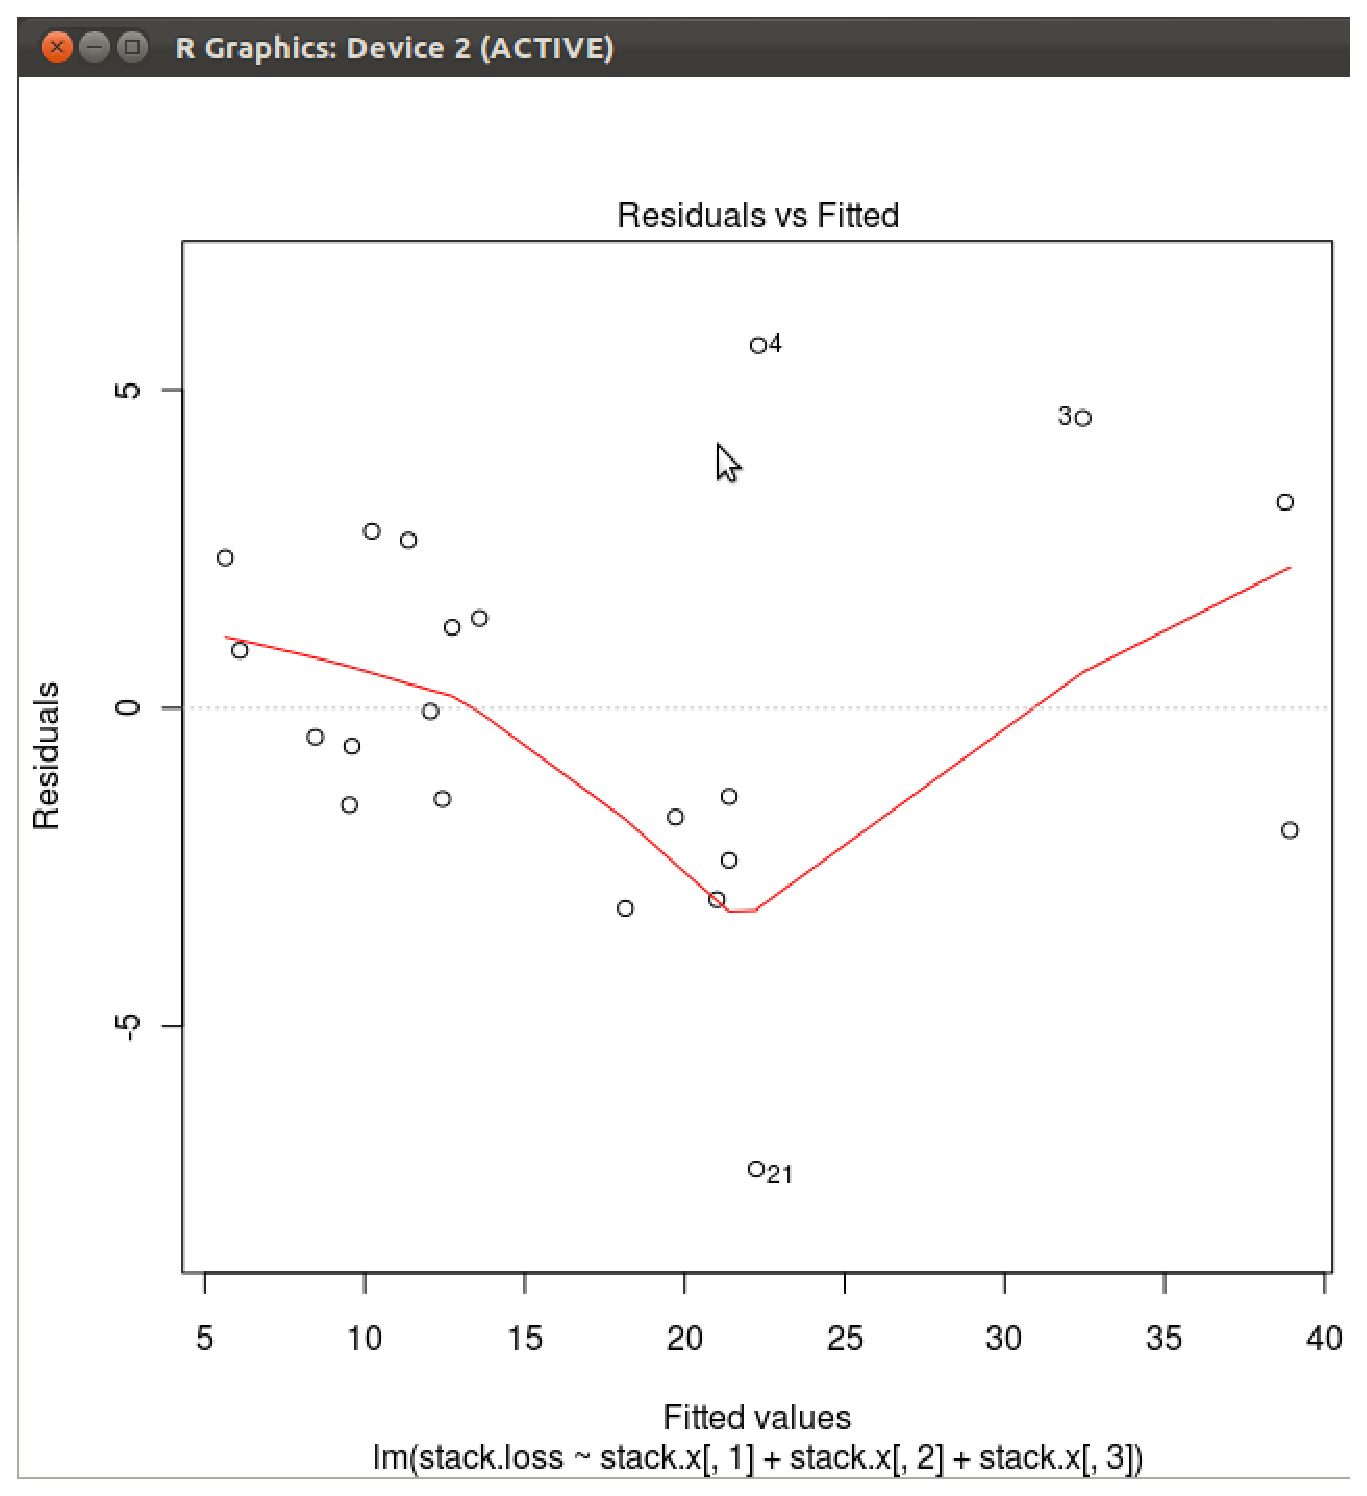
\includegraphics[width=0.7\textwidth]{p2-RvsF}
  \caption{Problem 2-a: Residual vs Fitted \label{fig:p2-RvsF}}
\end{figure}

About uncorrelated error, I use Perason's product-moment test to do
the analysis. And here is the result from R:

\begin{verbatim}
	Pearson's product-moment correlation

data:  stack.loss and stack.x[, 1] 
t = 10.2079, df = 19, p-value = 3.774e-09
alternative hypothesis: true correlation is not equal to 0 
95 percent confidence interval:
 0.8092570 0.9673185 
sample estimates:
      cor 
0.9196635 

	Pearson's product-moment correlation

data:  stack.loss and stack.x[, 2] 
t = 7.8977, df = 19, p-value = 2.028e-07
alternative hypothesis: true correlation is not equal to 0 
95 percent confidence interval:
 0.7134686 0.9486536 
sample estimates:
      cor 
0.8755044 

	Pearson's product-moment correlation

data:  stack.loss and stack.x[, 3] 
t = 1.9014, df = 19, p-value = 0.07252
alternative hypothesis: true correlation is not equal to 0 
95 percent confidence interval:
 -0.03850282  0.70912123 
sample estimates:
      cor 
0.3998296 
\end{verbatim}

As we can see, all three explanatory variables -- ``Air Flow'',
``Water Temp'' and ``Acid Conc'' are correlated with ``stack.loss''.\\

About outliers, here is the studentized deleted residuals from R:

\begin{verbatim}
          1           2           3           4           5           6 
 1.20947467 -0.70513857  1.61790411  2.05179748 -0.53050364 -0.96320379 
          7           8           9          10          11          12 
-0.82594672 -0.47365206 -1.04858585  0.42618802  0.87829204  0.96670672 
         13          14          15          16          17          18 
-0.46873058 -0.01695002  0.80061639  0.29118502 -0.59958579 -0.14868029 
         19          20          21 
-0.19719938  0.44311701 -3.33049332
\end{verbatim}

As we can see, only $|T_{21}| = 3.33 > t_{.975, 17} = 2.110$. So only
example 21 is an outlier.\\

About influential points, here is the DFFITS from R:

\begin{verbatim}
          1           2           3           4           5           6 
 0.79472051 -0.48132296  0.74415820  0.78788445 -0.12452440 -0.27915632 
          7           8           9          10          11          12 
-0.43767228 -0.25099001 -0.42339897  0.21312348  0.37621097  0.50917672 
         13          14          15          16          17          18 
-0.20268896 -0.00862896  0.38834173  0.11309290 -0.50202110 -0.06503243 
         19          20          21 
-0.09067758  0.13083298 -2.10029635 
\end{verbatim}

As we can see, only $|DFFITS_{21}| > 1$. So only example 21 is influential.

\appendix
\appendixpage
\addappheadtotoc

The code is listed below:

\verbatiminput{hmwk4.r}

\end{document} 
